\begin{figure}[!hp]
  \begin{center}
      \begin{tikzpicture}
        \begin{axis}[
            %colorbar,
            hide axis,
            scale only axis,
            height=0.26\rasterimagewidth,,
            width=\rasterimagewidth,
            %colorbar horizontal,
            point meta min=2.54,
            point meta max=3.08,
            colorbar style={
              title=Concentration [\%w],
              width=7.4cm,
              height=0.3cm,
              xtick={2.54, 2.75 3, 3.08, 3.5, 4, 4.5, 5, 5.5, 6},
              at={(0.5\rasterimagewidth,0.4cm)},
              anchor=north
            }
          ]
          \addplot [] coordinates {(0,0)};
          \node (myfirstpic) at (0,0) {\framebox{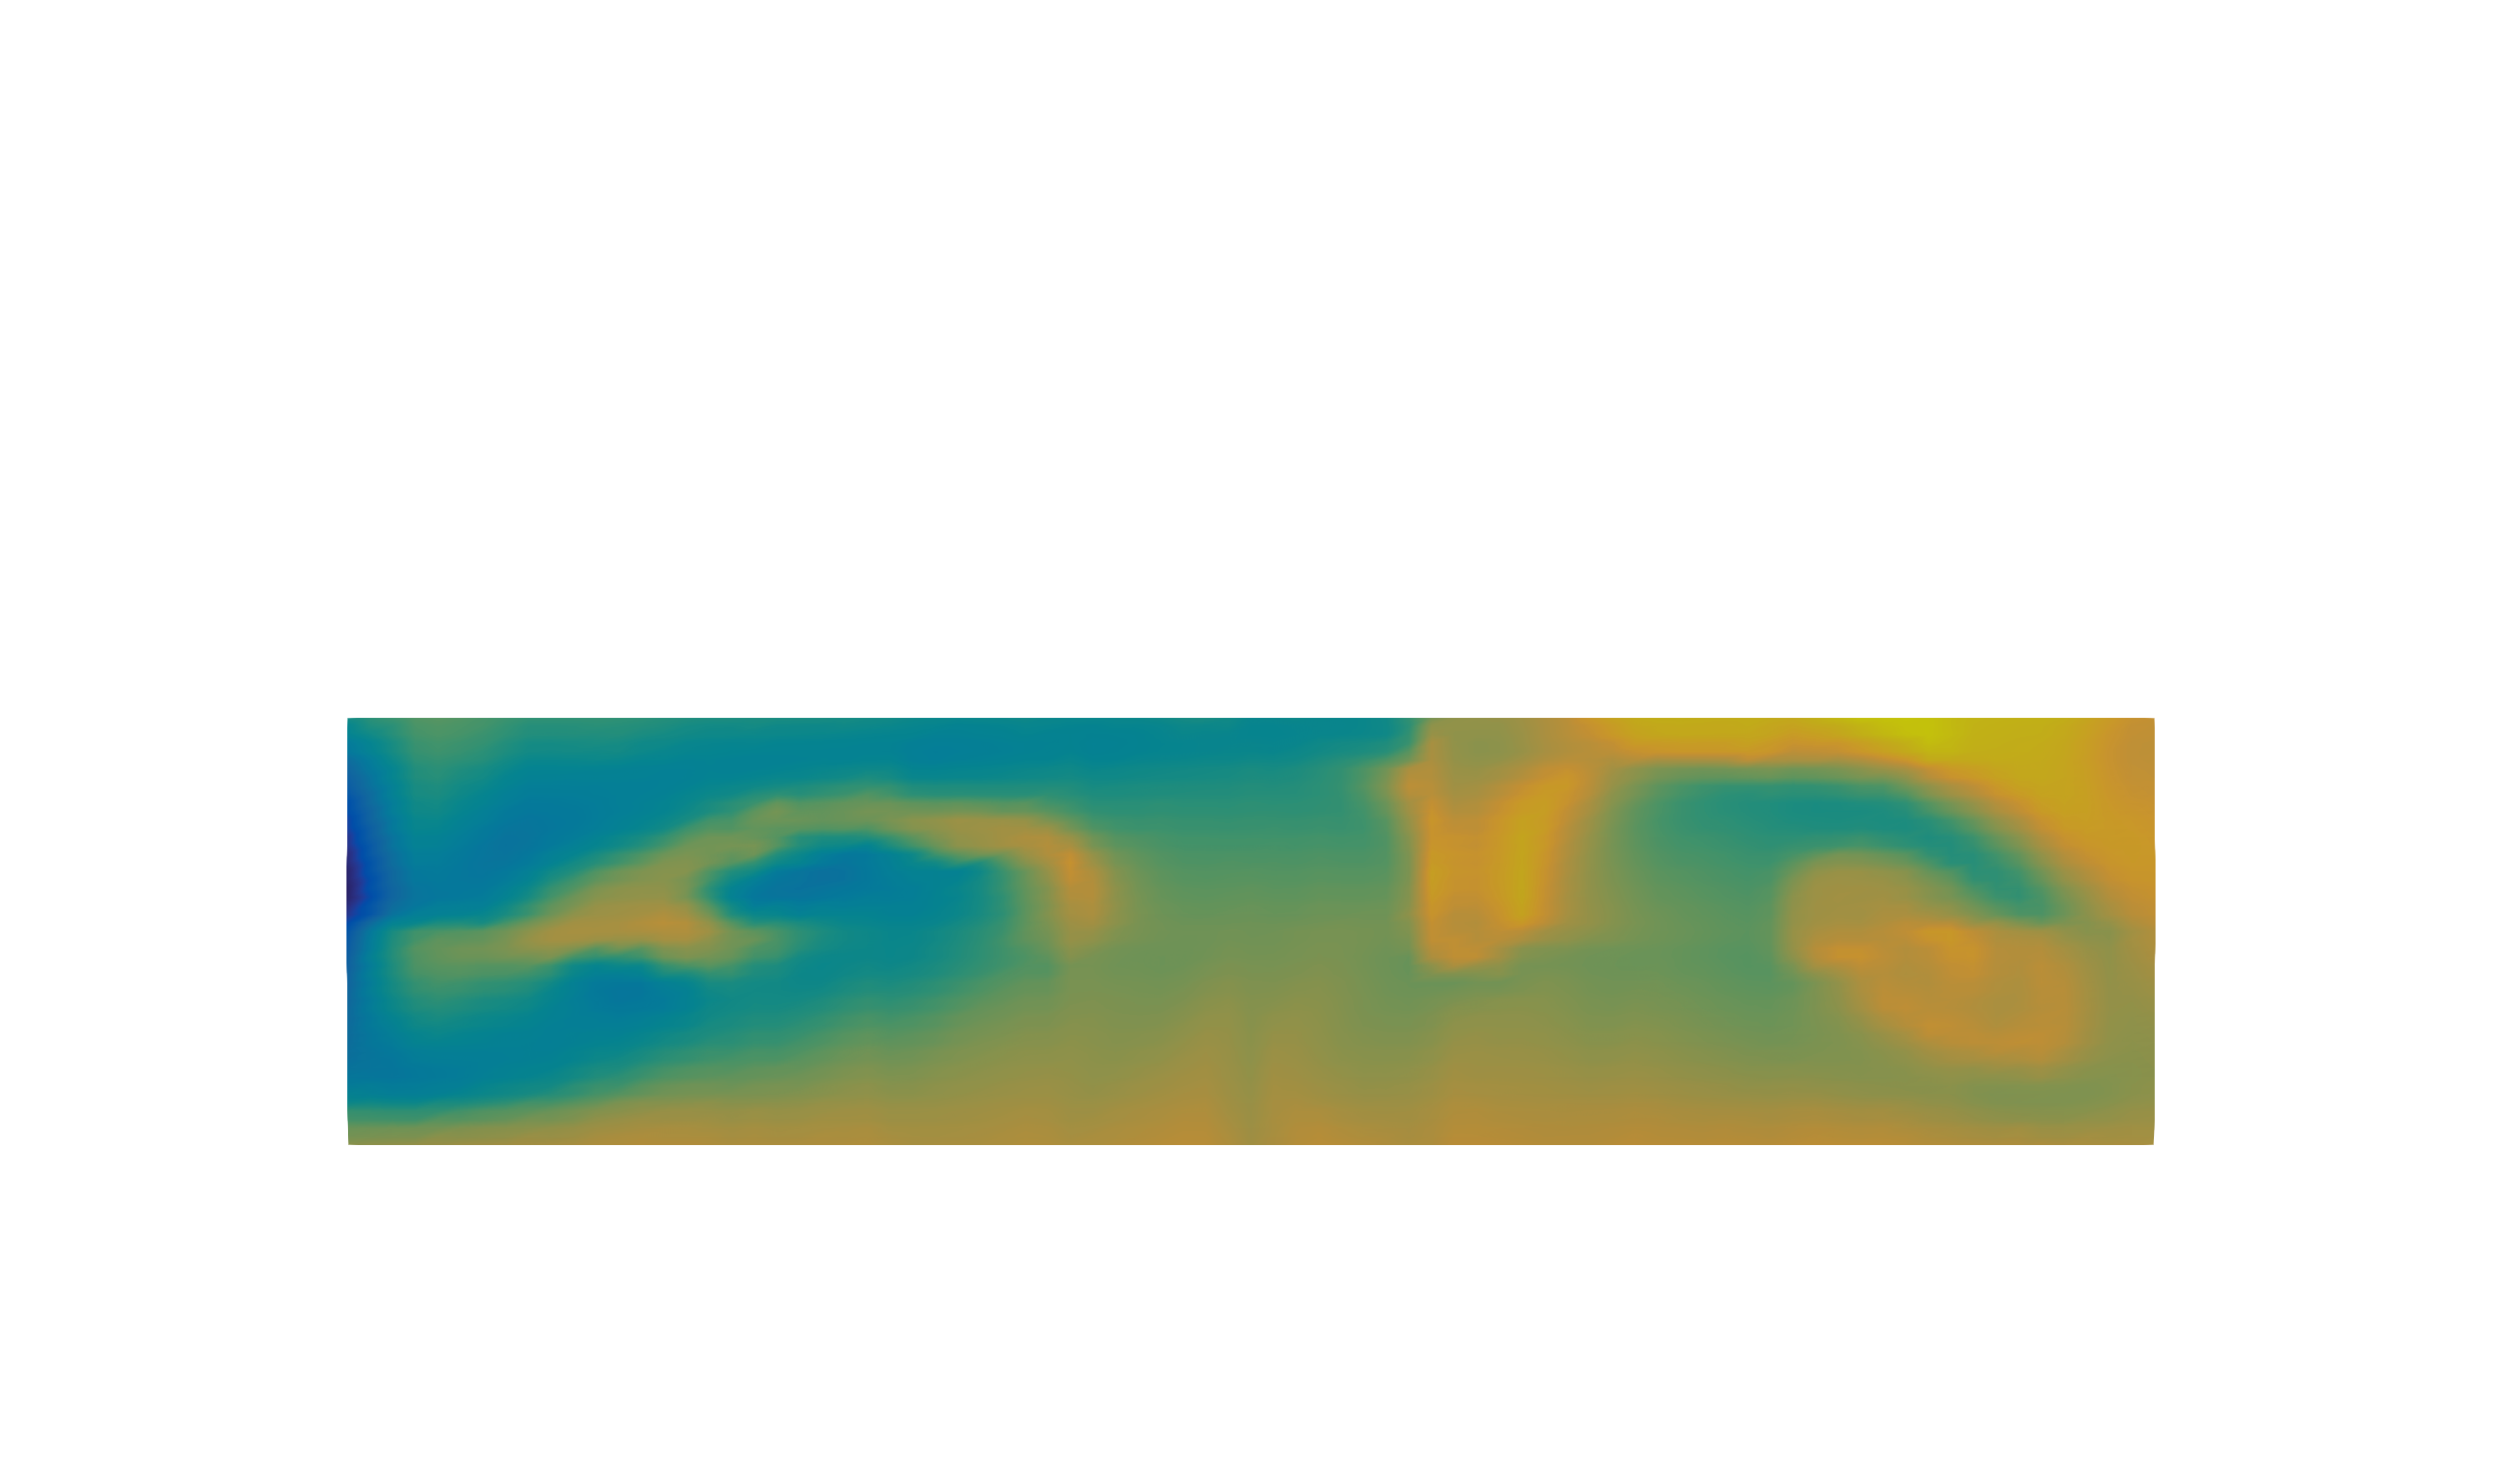
\includegraphics[width=\rasterimagewidth]{{../media/populations/application/print/alumina-influance-th1-2.54-3.08}.png}}};
        \end{axis}
      \end{tikzpicture}
      \begin{tikzpicture}
        \begin{axis}[
            %colorbar,
            hide axis,
            scale only axis,
            height=0.26\rasterimagewidth,,
            width=\rasterimagewidth,
            %colorbar horizontal,
            point meta min=2.54,
            point meta max=3.09,
            colorbar style={
              title=Concentration [\%w],
              width=7.4cm,
              height=0.3cm,
              xtick={2.54,2.75, 3,3.09, 3.5, 4, 4.5, 5, 5.5, 6},
              at={(0.5\rasterimagewidth,0.4cm)},
              anchor=north
            }
          ]
          \addplot [] coordinates {(0,0)};
          \node (myfirstpic) at (0,0) {\framebox{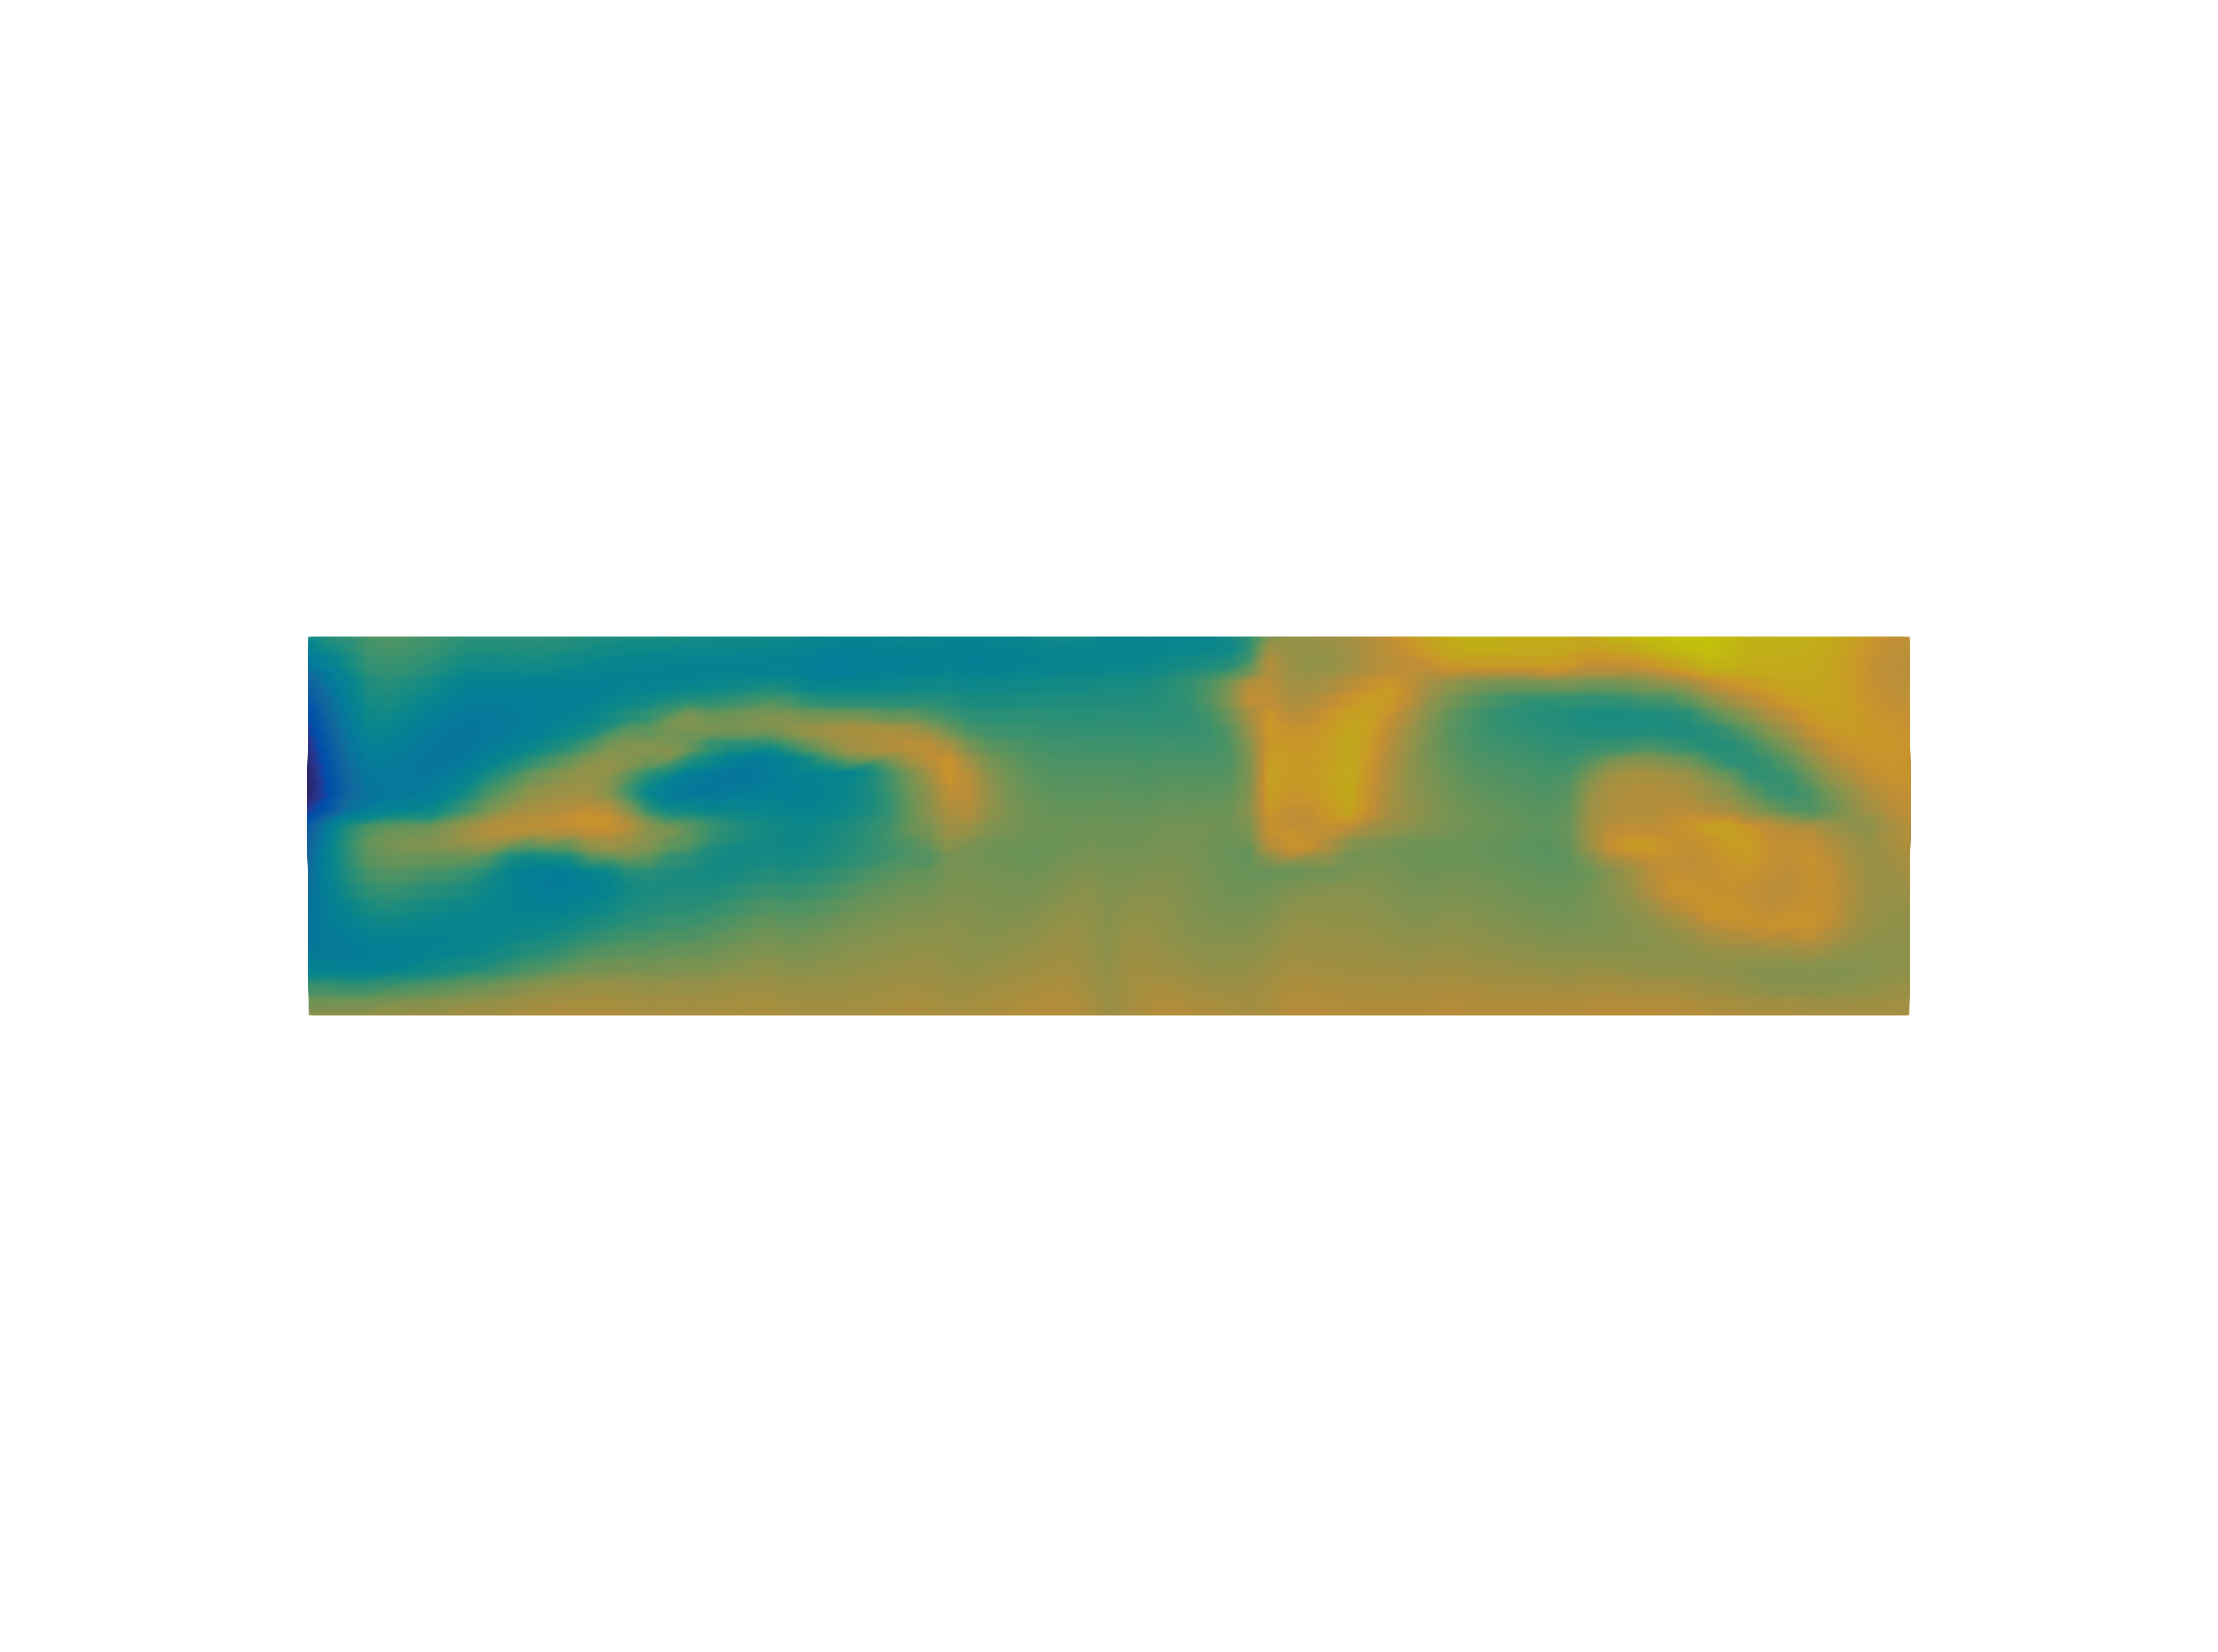
\includegraphics[width=\rasterimagewidth]{{../media/populations/application/print/alumina-influance-th2-2.54-3.09}.png}}};
        \end{axis}
      \end{tikzpicture}
      \begin{tikzpicture}
        \begin{axis}[
            %colorbar,
            hide axis,
            scale only axis,
            height=0.26\rasterimagewidth,,
            width=\rasterimagewidth,
            %colorbar horizontal,
            point meta min=2.54,
            point meta max=3.09,
            colorbar style={
              title=Concentration [\%w],
              width=7.4cm,
              height=0.3cm,
              xtick={2.54, 2.75, 3, 3.09, 3.5, 4, 4.5, 5, 5.5, 6},
              at={(0.5\rasterimagewidth,0.4cm)},
              anchor=north
            }
          ]
          \addplot [] coordinates {(0,0)};
          \node (myfirstpic) at (0,0) {\framebox{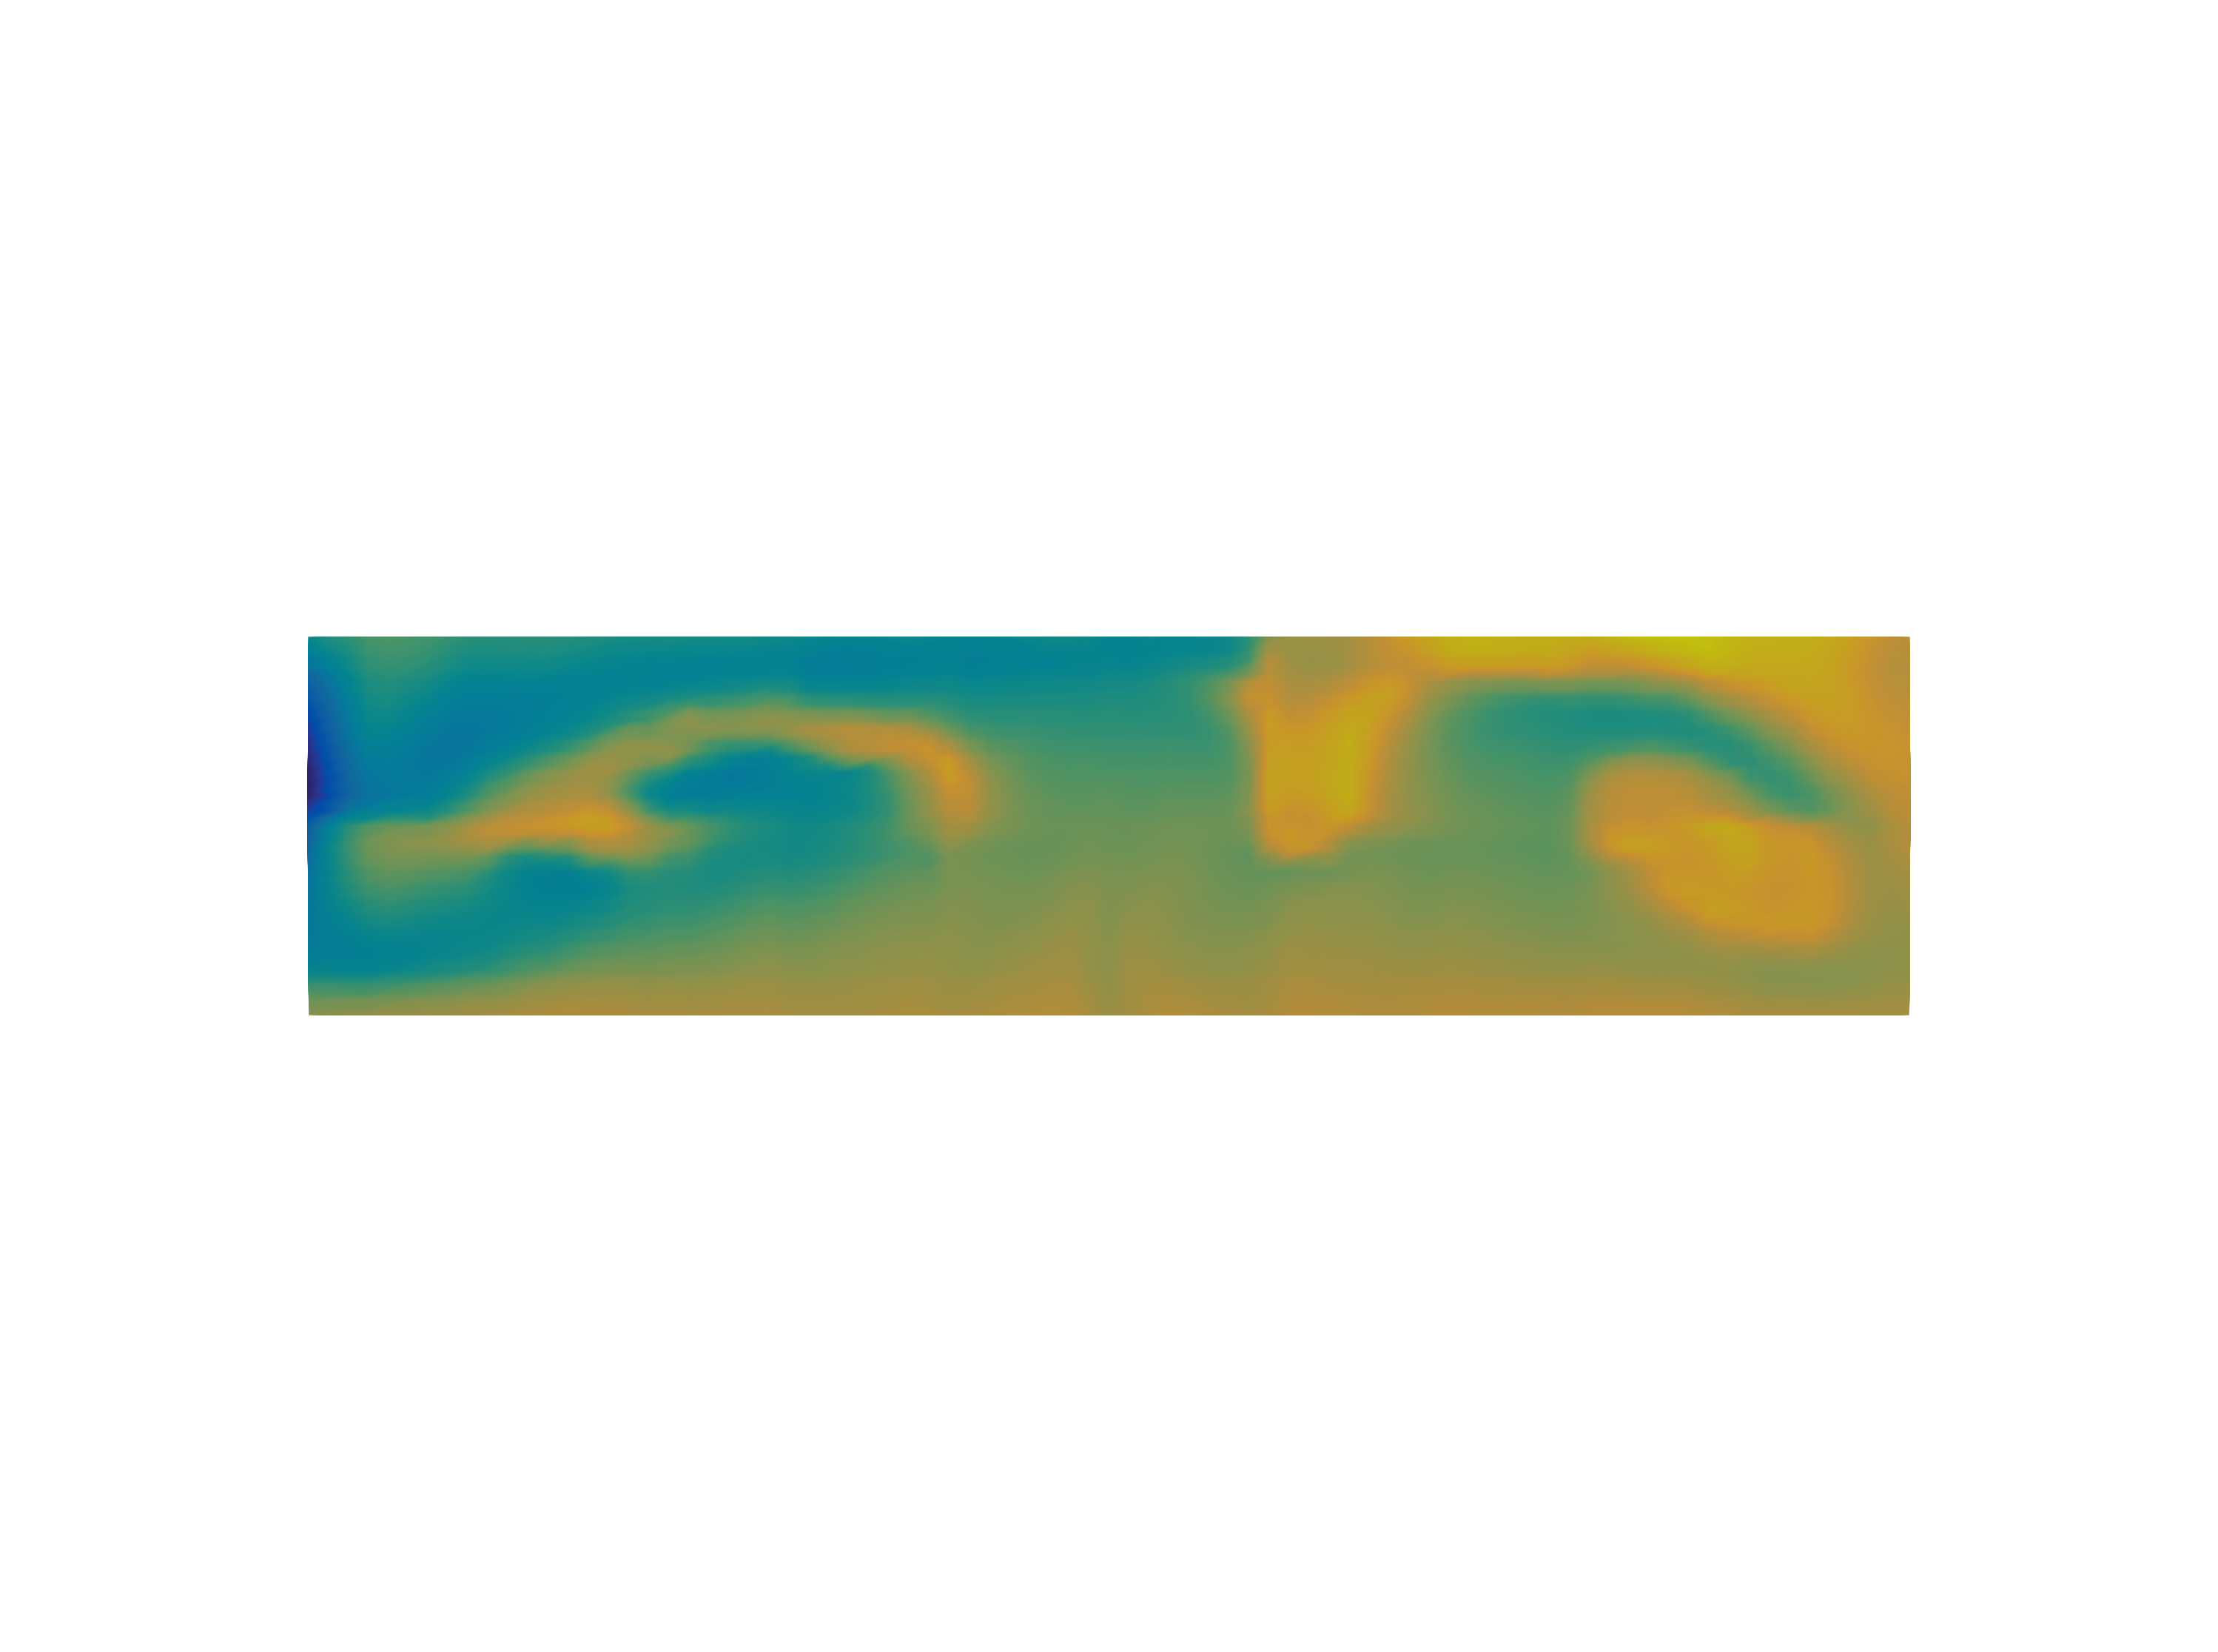
\includegraphics[width=\rasterimagewidth]{{../media/populations/application/print/alumina-influance-th5-2.54-3.09}.png}}};
        \end{axis}
      \end{tikzpicture}
      \begin{tikzpicture}
        \begin{axis}[
            colorbar,
            hide axis,
            scale only axis,
            height=0.52\rasterimagewidth,,
            width=\rasterimagewidth,
            colorbar horizontal,
            point meta min=2.54,
            point meta max=3.09,
            colorbar style={
              title=Concentration [\%w],
              width=7.4cm,
              height=0.3cm,
              xtick={2.54,2.75, 3, 3.09, 3.5, 4, 4.5, 5, 5.5, 6},
              at={(0.5\rasterimagewidth,3.0cm)},
              anchor=north
            }
          ]
          \addplot [] coordinates {(0,0)};
          \node (myfirstpic) at (0,50) {{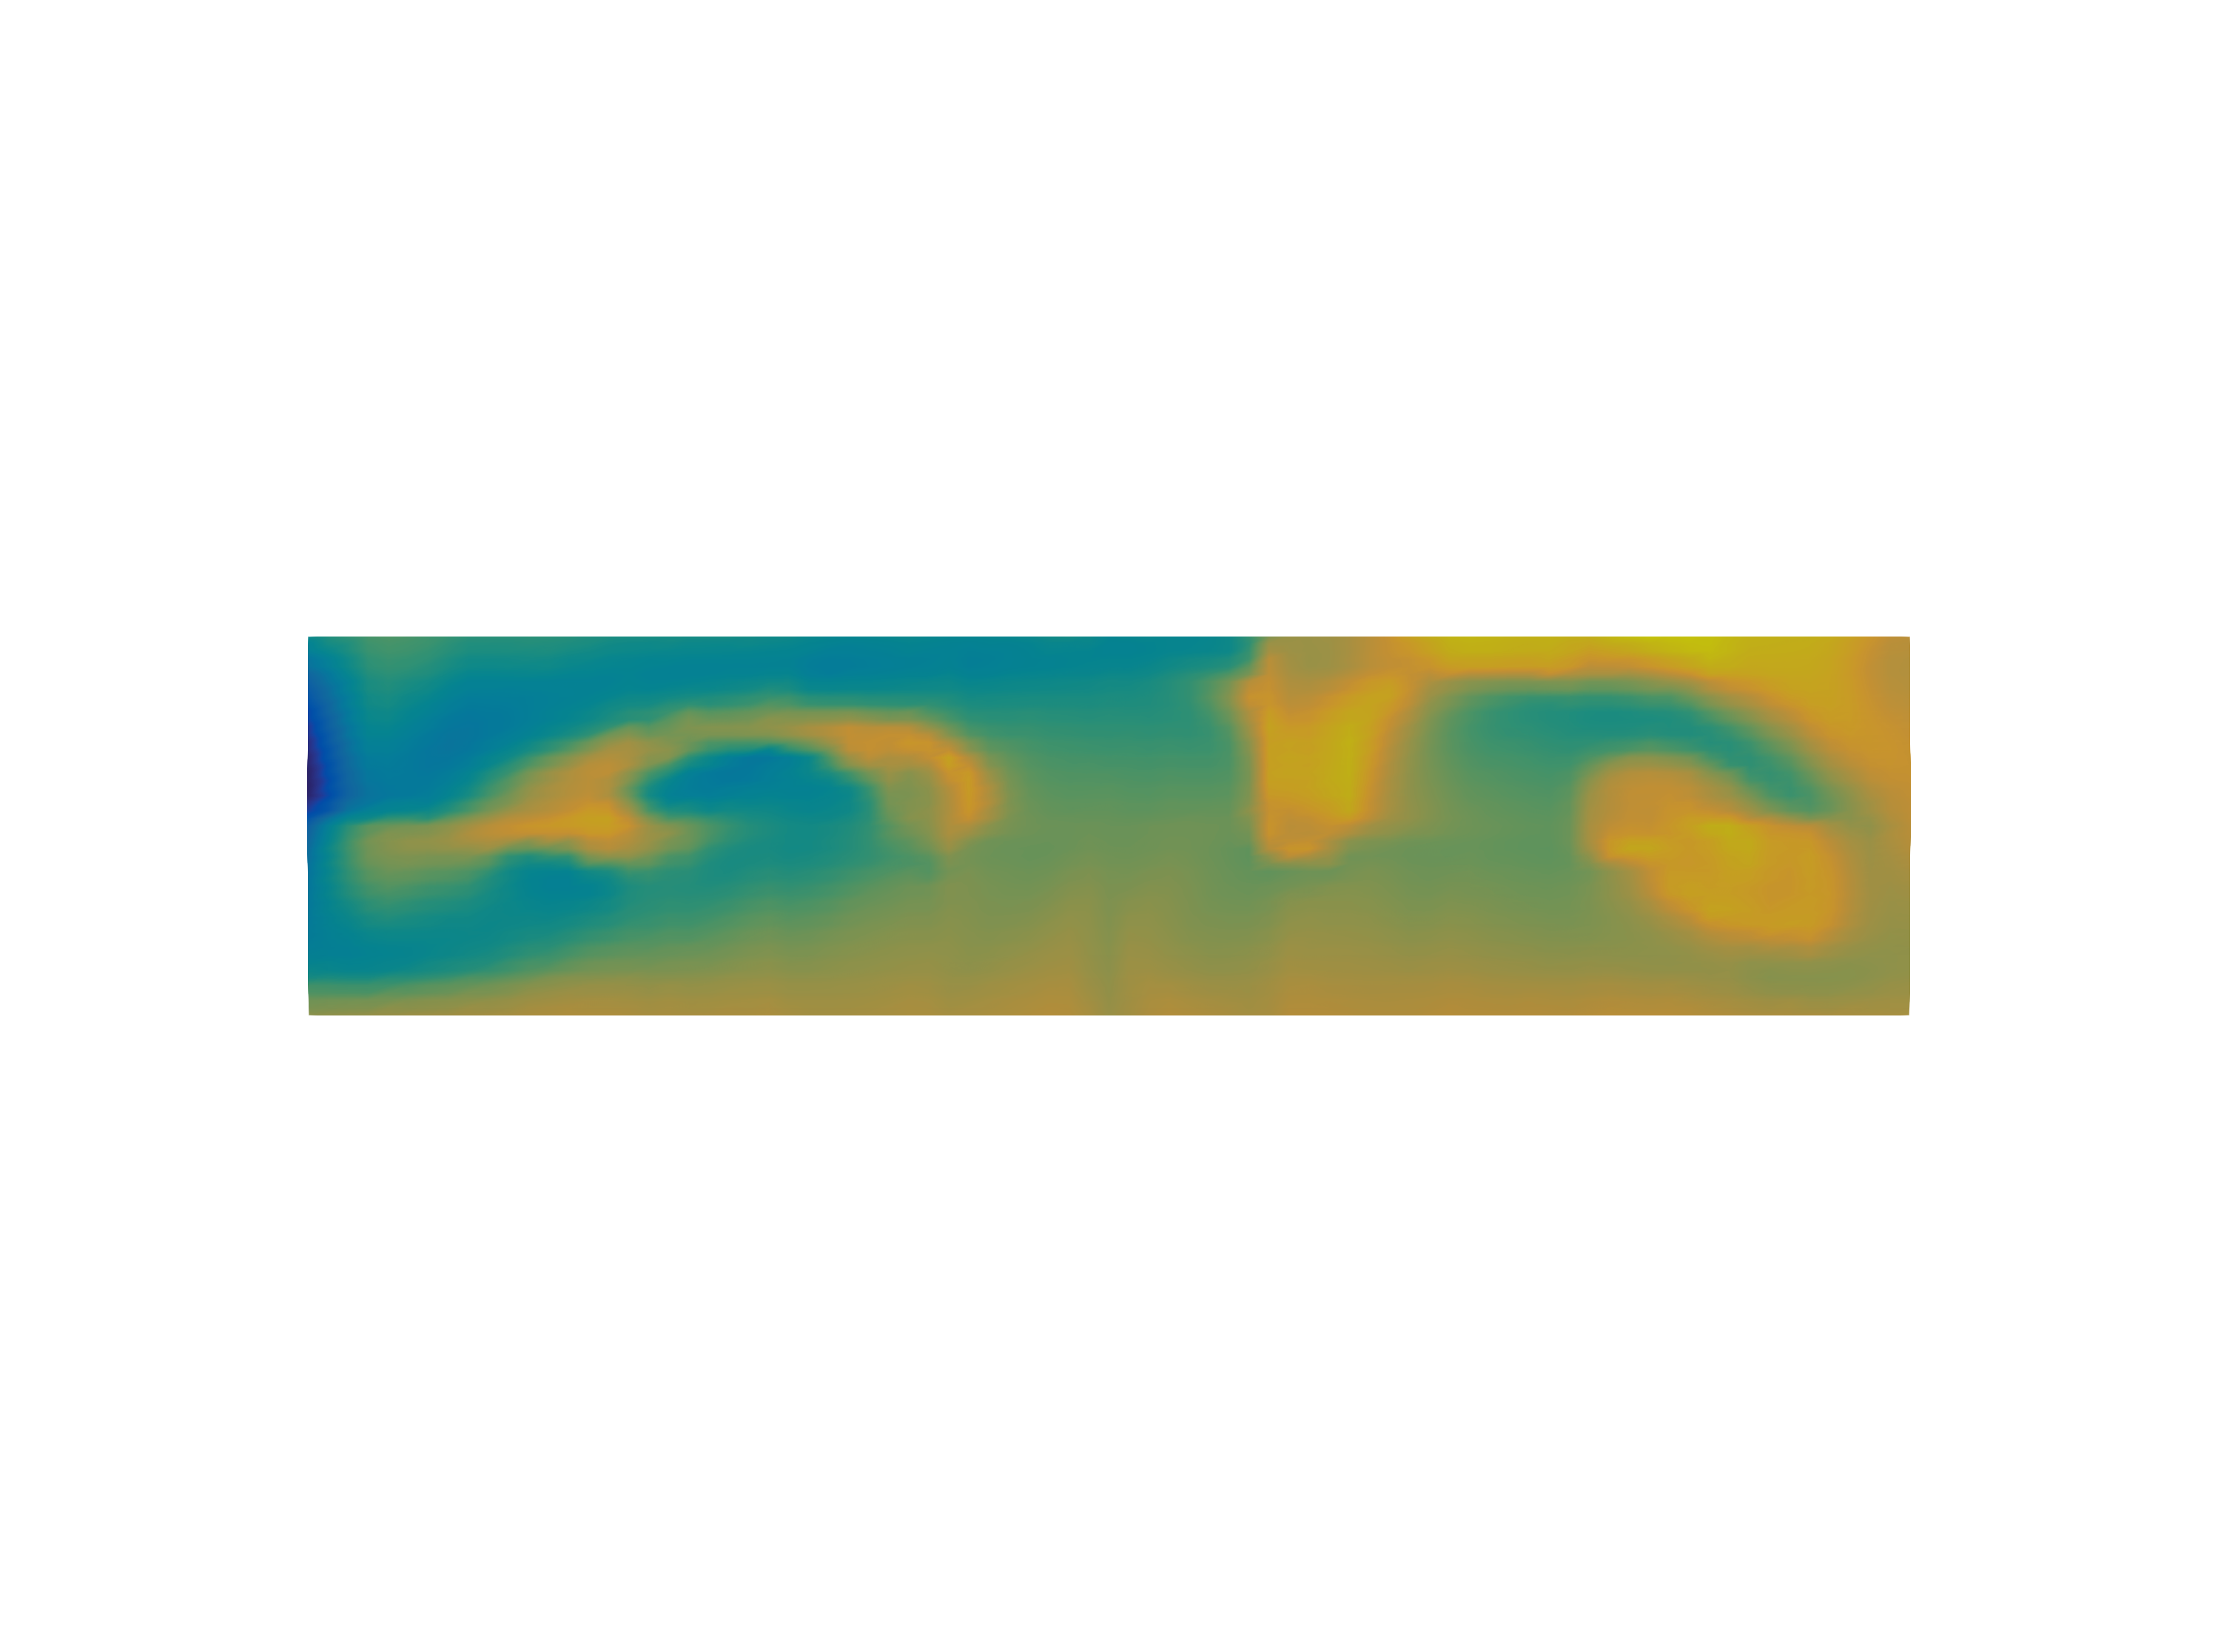
\includegraphics[width=\rasterimagewidth]{{../media/populations/application/print/alumina-influance-th510-2.54-3.09}.png}}};
        \end{axis}
      \end{tikzpicture}
    \caption{Champ de concentration $c$ dans l'ACD de la cuve AP32 à
      $t = \num{10000}$ \si{second}. De haut en bas, le temps de
      latence de dissolution $T_\text{Lat} = 1\si\second$,
      $2\si\second$, $5\si\second$ et $10\si\second$.}
    \label{fig:dissolution-alumin-influence-tlat}
  \end{center}
\end{figure}
